\documentclass{beamer}
\usepackage{microtype}
\usepackage{siunitx}
\usepackage{graphicx}
\usepackage[backend=biber, style=numeric]{biblatex}
\addbibresource{presentation-warning-signs.bib}
\setbeamertemplate{frametitle continuation}{\space(\insertcontinuationcount)}

\title{Climate change --- tropical storms}
\author{Manasvi Sharma \and Ahaan Shokeen}
\date{2026-04-07}

\begin{document}

\maketitle

\begin{frame}
    \frametitle{What is happening?}
    \begin{itemize}
        \item Tropical storms are becoming more intense and destructive in many regions due to global warming.
        \item Scientists have found that the strongest tropical cyclones are increasing in intensity, and climate change is most probably the cause behind it.
        \item \textbf{What normally happens:} Tropical storms form over warm water --- \qty{299.15}{\kelvin}--\qty{310.15}{\kelvin} (\qty{26}{\degreeCelsius}--\qty{37}{\degreeCelsius}). They gain energy slowly and follow mostly predictable paths, and weaken before reaching land.
        \item \textbf{What is happening now:} Due to rising temperatures, storms are getting more energy and are strengthening very quickly, even within hours, there is heavier rainfall due to warmer weather holding more moisture, which leads to flooding. It’s making them more intense, dangerous, and unpredictable.
        \item Tropical storms typically have speeds of \qty{17}{\metre\per\second}--\qty{28}{\metre\per\second}, but climate change is making them faster.
    \end{itemize}
\end{frame}

\begin{frame}
    \frametitle{Why is it happening?}
    Human activites \textrightarrow{} greenhouse gases emitted \textrightarrow{} more heat in the atmosphere \textrightarrow{} oceans absorb 90\% of this heat \textrightarrow{} more thermal energy for storms to draw on \textrightarrow{} increased moisture \textrightarrow{} intense precipitation (rain, snow, sleet, hail, etc.), intense convection \textrightarrow{} stronger wind.

    \vspace{5mm}
    Essentially, it's the humans again ruining everything.

\end{frame}

\begin{frame}
    \frametitle{How shall it affect the future?}
    \begin{itemize}
        \item Coastal cities at risk --- flooding and infrastructure damage due to natural disasters.
        \item Repeated destruction --- communities cannot rebuild sustainably.
        \item Loss of natural barriers such as mangroves and coral reefs --- less protection against more storms.
        \item Economic strain --- the destruction of the cities will strain the cities to their economic limit, especially developing cities.
        \item Increase in climate-based migration --- temporary/permanent migration of people due to unfavourable climatic conditions or environmental destruction.
        \item Stronger storms destroy resources faster than they can recover, which makes long term human survival in a few regions unsustainable.
    \end{itemize}
\end{frame}

\begin{frame}
    \frametitle{Photographic evidence}
    \begin{columns}
        \begin{column}{40mm}
            \begin{figure}
                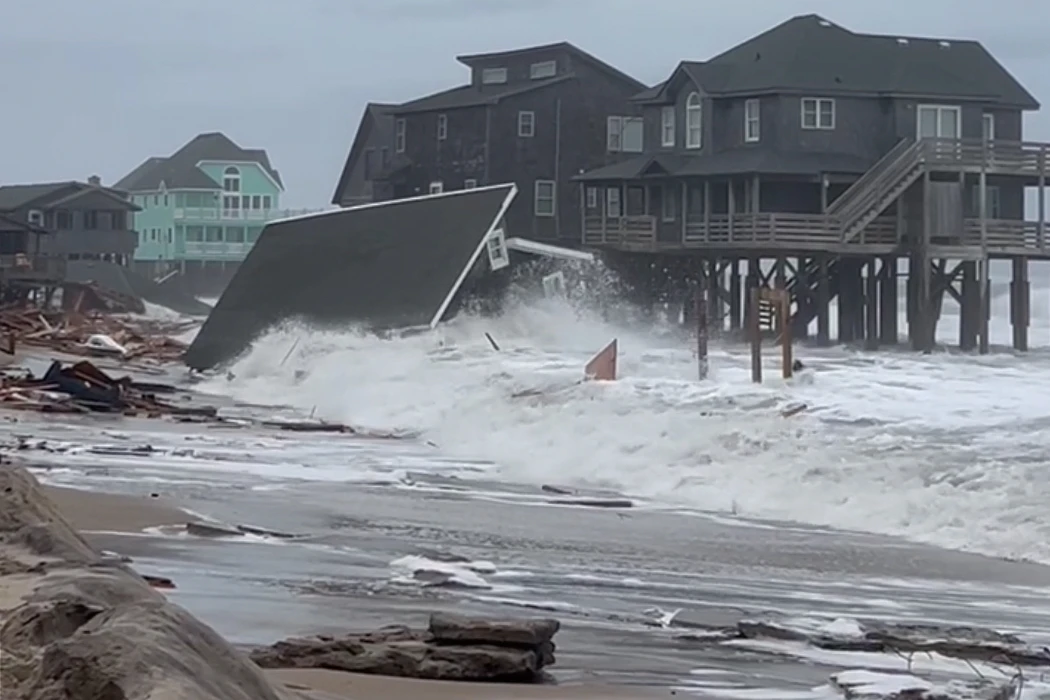
\includegraphics[width=40mm]{images/ap-news-hurricane.png}
                \caption{\cite{robertson-2025}}
            \end{figure}
            \begin{figure}
                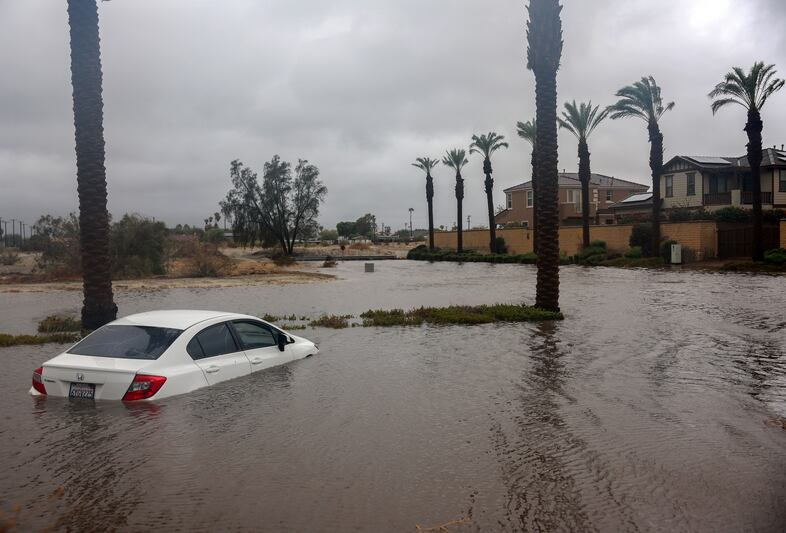
\includegraphics[width=40mm]{images/opb-hilary.jpg}
                \caption{\cite{werbeck-2023}}
            \end{figure}
        \end{column}
        \begin{column}{40mm}
            \begin{figure}
                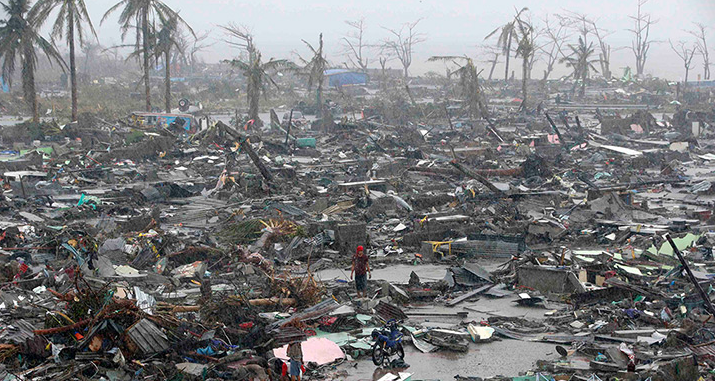
\includegraphics[width=40mm]{images/ee-tropical-cyclones.png}
                \caption{\cite{frank-2025}}
            \end{figure}
            \begin{figure}
                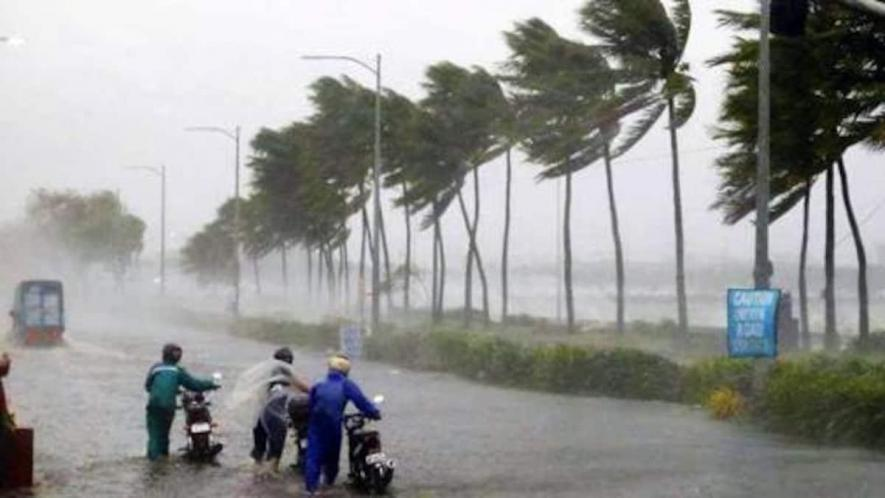
\includegraphics[width=40mm]{images/earth-warming-cyclone-grow.jpg}
                \caption{\cite{talukdar-2020}}
            \end{figure}
        \end{column}
    \end{columns}
\end{frame}

\begin{frame}
    \frametitle{Graphs to be analysed}
    \begin{columns}
        \begin{column}{60mm}
            \begin{figure}
                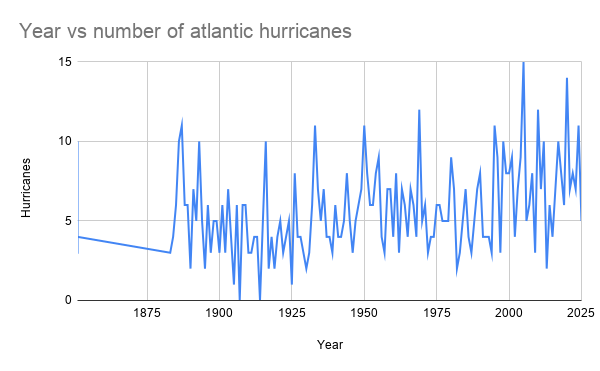
\includegraphics[width=60mm]{images/atlantic-hurricanes-per-year-graph-linear.png}
                \caption{A linear graph using the data from \cite{hurricane-year}}
            \end{figure}
        \end{column}
        \begin{column}{60mm}
            \begin{figure}
                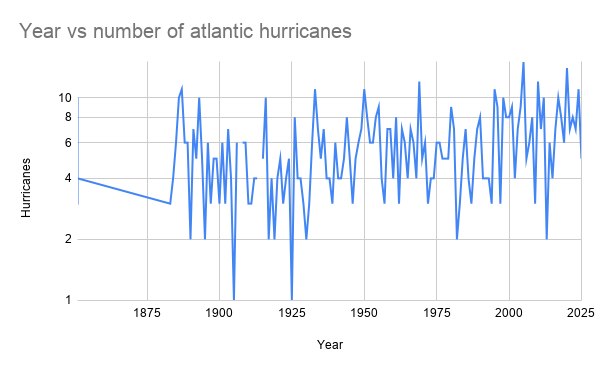
\includegraphics[width=60mm]{images/atlantic-hurricane-per-year-graph-log.png}
                \caption{A logarithmic graph using the data from \cite{hurricane-year}}
            \end{figure}
        \end{column}
    \end{columns}
\end{frame}

\begin{frame}[allowframebreaks]
    \frametitle{Works Cited}
    \printbibliography
\end{frame}

\end{document}